\documentclass[aspectratio=169]{beamer}
\usepackage[UTF8]{ctex}
\usepackage[T1]{fontenc}
\usepackage{amsmath,amssymb,bm}
\usepackage{booktabs}
\usepackage{graphicx}
\usepackage{array}
\usepackage{xcolor}
\usepackage{hyperref}
\usepackage{PekingU}

\graphicspath{{figures/}{pic/}}
\setlength{\parindent}{0pt}
\setbeamertemplate{caption}[numbered]

\definecolor{baselinecolor}{RGB}{127,0,0}
\definecolor{tunedcolor}{RGB}{184,115,0}
\definecolor{variantcolor}{RGB}{92,105,117}
\definecolor{sourcegray}{RGB}{95,95,95}

\title{Predicting LLM Pretraining Loss Curves Across Learning-Rate Schedules}
\subtitle{Revisiting the capacity of MTL through a broader parameter search}
\author{Group members: 黄天域, 王梓桐, 柯怿憬}
\institute{Peking University}
\date{June 19, 2026}

\newcommand{\best}[1]{\textbf{#1}}
\newcommand{\second}[1]{\emph{#1}}
\newcommand{\source}[1]{\vfill{\tiny\color{sourcegray}#1}}

\begin{document}

\begin{frame}
  \titlepage
\end{frame}

\begin{frame}{Roadmap}
  The presentation follows the scientific argument in four stages.
  \begin{enumerate}
    \item We formulate schedule-to-loss prediction and introduce three published baselines: MTL, MPL, and FSL.
    \item We develop \textbf{Tuned-MTL}, our main contribution, by expanding the memory-scale search and revising the fitting emphasis.
    \item We evaluate all methods under a common cosine-to-WSD protocol and interpret their prediction curves.
    \item We summarize several smaller exploratory variants and the broader lessons from the comparison.
  \end{enumerate}
\end{frame}

\section{Problem Formulation}

\begin{frame}{Why Predict an Entire Loss Curve?}
  A full pretraining run is expensive, while schedule decisions must often be made before that run is available.
  \begin{itemize}
    \item A loss-curve model estimates training progress under a candidate learning-rate schedule.
    \item Curve prediction reveals when two schedules begin to diverge, rather than reporting only their final losses.
    \item A transferable model can support schedule design using a small number of observed training curves.
  \end{itemize}
  \vspace{0.35em}
  The central difficulty is historical dependence: the loss at step \(t\) reflects the complete optimization path up to that step.
\end{frame}

\begin{frame}{Schedule-to-Loss Prediction}
  For a training horizon \(T\), let
  \[
    \bm{\eta}=(\eta_1,\eta_2,\ldots,\eta_T)^\top
  \]
  denote the learning-rate schedule. We model the loss at step \(t\) as a functional of the schedule prefix:
  \[
    L_t=L_{\Theta}(\eta_{\leq t}),
    \qquad
    \eta_{\leq t}=(\eta_1,\eta_2,\ldots,\eta_t).
  \]
  The parameters \(\Theta\) are fitted from an observed curve. Transfer requires the same fitted functional to predict a curve produced by a different schedule.
\end{frame}

\begin{frame}{Course Task and Research Question}
  The main experiment fits each method on the loss curve produced by a cosine schedule and evaluates its prediction on a warmup-stable-decay (WSD) schedule.
  \[
    \text{cosine curve for fitting}
    \quad\longrightarrow\quad
    \text{WSD curve for evaluation}.
  \]
  A three-stage \(8\)-\(1\)-\(1\) schedule provides a second, auxiliary transfer case.
  \vspace{0.6em}

  \textbf{Research question.} How much of the observed transfer performance comes from adding model complexity, and how much remains available inside the parameter space of the earliest MTL baseline?
\end{frame}

\section{Published Baselines}

\begin{frame}{Three Baseline Perspectives}
  The three published methods encode schedule history in different ways.
  \begin{center}
  \small
  \begin{tabular}{p{0.16\linewidth}p{0.31\linewidth}p{0.39\linewidth}}
    \toprule
    Method & Central object & Intuition \\
    \midrule
    MTL & exponentially decaying memory & summarize learning-rate changes with one persistent state \\
    MPL & a sum of power-law responses & treat each learning-rate decrease as a source with its own delayed effect \\
    FSL & intrinsic time and convolution & measure progress by accumulated learning rate and convolve past schedule changes \\
    \bottomrule
  \end{tabular}
  \end{center}
  These perspectives provide increasingly expressive descriptions of schedule response, with correspondingly different data requirements.
\end{frame}

\begin{frame}{Baseline 1: Momentum Law (MTL)}
  MTL models the predicted loss as
  \[
    \widehat L_t
    =
    L_0 + A T_t^{-\alpha} - C S_2(t),
    \qquad
    T_t=\epsilon+\sum_{i\leq t}\eta_i .
  \]
  \begin{itemize}
    \item \(L_0+A T_t^{-\alpha}\) is a power law in accumulated learning rate, which acts as a measure of training progress.
    \item \(C S_2(t)\) represents the additional loss reduction associated with learning-rate annealing.
    \item The model uses four continuous parameters and one memory parameter, \(\lambda\).
  \end{itemize}
  \source{Tissue, Wang, and Wang, \emph{Scaling Law with Learning Rate Annealing}, arXiv:2408.11029, 2024.}
\end{frame}

\begin{frame}{MTL Memory and Parameter Meanings}
  The annealing state obeys
  \[
    m_t=\lambda m_{t-1}+(\eta_{t-1}-\eta_t),
    \qquad
    S_2(t)=\sum_{i\leq t}m_i .
  \]
  A learning-rate decrease creates a positive impulse. The factor \(\lambda\) controls how slowly that impulse fades.
  \begin{center}
  \small
  \begin{tabular}{cl}
    \toprule
    Parameter & Interpretation \\
    \midrule
    \(L_0\) & asymptotic loss floor \\
    \(A,\alpha\) & scale and exponent of the progress term \\
    \(C\) & magnitude of the annealing contribution \\
    \(\lambda\) & persistence of schedule memory; values near one retain longer history \\
    \bottomrule
  \end{tabular}
  \end{center}
  \source{Tissue, Wang, and Wang, arXiv:2408.11029, 2024.}
\end{frame}

\begin{frame}{Baseline 2: Multi-Power Law (MPL)}
  MPL associates every positive learning-rate decrease
  \[
    \Delta_i^+=\max(\eta_{i-1}-\eta_i,0)
  \]
  with a delayed power-law response:
  \[
  \widehat L_t=L_0+A T_t^{-\alpha}
  -B\sum_{i\leq t}\Delta_i^+
  \left[
    1-\left(1+C\eta_i^{-\gamma}(T_t-T_i+\eta_i)\right)^{-\beta}
  \right].
  \]
  The total schedule effect is the sum of these responses. MPL can therefore represent different effects for the timing and magnitude of multiple decay events.
  \source{Luo et al., \emph{A Multi-Power Law for Loss Curve Prediction Across Learning Rate Schedules}, arXiv:2503.12811, 2025.}
\end{frame}

\begin{frame}{How to Read the MPL Parameters}
  MPL retains the progress term from MTL and adds a flexible response kernel.
  \begin{itemize}
    \item \(L_0\), \(A\), and \(\alpha\) describe the loss floor and the power-law improvement with accumulated learning rate.
    \item \(B\) scales the total benefit assigned to learning-rate decreases.
    \item \(C\) sets the response timescale, while \(\beta\) controls the response shape.
    \item \(\gamma\) changes the response according to the learning rate at which a decrease occurs.
  \end{itemize}
  \vspace{0.35em}
  The additional flexibility can distinguish several decay events, although estimating seven coupled parameters from one fitting curve is statistically demanding.
  \source{Luo et al., arXiv:2503.12811, 2025.}
\end{frame}

\begin{frame}{Baseline 3: Functional Scaling Laws (FSL)}
  Functional Scaling Laws define training progress through intrinsic time:
  \[
    T(k)=\sum_{i\leq k}\eta_i .
  \]
  Two training steps with different learning rates therefore represent different amounts of progress. The practical loss model has the form
  \[
    \widehat L_k=L_0+\frac{c_1}{T(k)^s}-\mathrm{LRD}(k),
  \]
  where \(\mathrm{LRD}(k)\) is a convolutional response to earlier learning-rate decreases.
  \source{Li, Chen, Huang, Wang, and Wu, \emph{Functional Scaling Laws in Kernel Regression}, arXiv:2509.19189, 2025.}
\end{frame}

\begin{frame}{FSL Schedule-Response Kernel}
  For fixed model and data size, the practical response used in our reproduction is
  \[
  \mathrm{LRD}(k)=
  c_2\sum_{i\leq k}\Delta_i^+
  \left(c_3+T(i)^{-s}\right)
  \left[
    1-\left(1+c_4(T(k)-T(i))\right)^{-\gamma}
  \right].
  \]
  \begin{itemize}
    \item \(c_1\) and \(s\) determine the progress law.
    \item \(c_2\) scales the combined schedule response, and \(c_3\) adjusts source strength.
    \item \(c_4\) and \(\gamma\) control how the effect of each decay event grows with intrinsic-time separation.
  \end{itemize}
  \source{Li et al., arXiv:2509.19189, 2025; practical LLM ansatz in Appendix B.2.}
\end{frame}

\begin{frame}{Baseline Comparison Before Tuning}
  \begin{center}
  \small
  \begin{tabular}{llll}
    \toprule
    Method & Schedule memory & Continuous parameters & Main inductive bias \\
    \midrule
    MTL & one exponential scale & four, plus \(\lambda\) & persistent state \\
    MPL & event-wise power response & seven & decay superposition \\
    FSL & intrinsic-time convolution & seven & convolutional kernel \\
    \bottomrule
  \end{tabular}
  \end{center}
  MTL is the oldest and lowest-dimensional method in this comparison. Its compact structure becomes valuable when only one curve is available for fitting.
\end{frame}

\section{Main Contribution: Tuned-MTL}

\begin{frame}{Central Finding: MTL Has Substantial Unused Capacity}
  The clean baseline comparison identifies MTL as the strongest of the three published methods under the one-curve fitting regime.
  \begin{itemize}
    \item The default MTL search examines only five values of \(\lambda\).
    \item Near \(\lambda=1\), a small numerical change produces a large change in memory duration.
    \item A sparse grid can therefore exclude the timescale needed for transfer to WSD.
  \end{itemize}
  \vspace{0.4em}
  Our main contribution is \textbf{Tuned-MTL}: an estimation procedure that searches a broader memory space and places greater fitting emphasis on the informative late portion of the cosine curve.
\end{frame}

\begin{frame}{Tuned-MTL Retains the Complete MTL Model}
  Tuned-MTL uses the same predictive equation:
  \[
    \widehat L_t
    =
    L_0+A\left(\epsilon+\sum_{i\leq t}\eta_i\right)^{-\alpha}
    -C\sum_{i\leq t}m_i,
    \qquad
    m_i=\lambda m_{i-1}+(\eta_{i-1}-\eta_i).
  \]
  The estimation procedure changes in three places:
  \begin{enumerate}
    \item the \(\lambda\) grid expands from five values to thirteen values concentrated near one;
    \item selected points in the final 20\% of the cosine curve receive weight \(3\), compared with weight \(2\) in the baseline fit;
    \item fifty random restarts explore the expanded grid, compared with twenty for the baseline.
  \end{enumerate}
\end{frame}

\begin{frame}{Why the Memory Search Matters}
  Exponential memory has an approximate half-life
  \[
    h_{1/2}=\frac{\log(1/2)}{\log\lambda}.
  \]
  \begin{center}
  \begin{tabular}{lrr}
    \toprule
    Fit & Selected \(\lambda\) & Approximate half-life \\
    \midrule
    Baseline MTL & \(0.99\) & \(69\) recorded steps \\
    Tuned-MTL & \(0.9997\) & \(2310\) recorded steps \\
    \bottomrule
  \end{tabular}
  \end{center}
  Tuned-MTL selects a much longer schedule memory. This allows an annealing event to influence predictions over a substantial fraction of training.
\end{frame}

\begin{frame}{What Tail Weighting Changes}
  Let
  \[
    r_t=\log\widehat L_t-\log \overline L_t
  \]
  be the residual against the smoothed cosine loss. Tuned-MTL minimizes
  \[
    \sum_{t\in I_{\mathrm{fit}}} w_t\,H_{\delta}(r_t),
    \qquad
    w_t=
    \begin{cases}
      3, & t\text{ lies in the final 20\% of the fitting region},\\
      1, & \text{otherwise}.
    \end{cases}
  \]
  Per selected point, late cosine observations contribute three times as strongly. Empirically, this emphasis helps identify the long-memory solution that transfers accurately across the full WSD curve.
\end{frame}

\begin{frame}{Selected Tuned-MTL Parameters}
  \begin{center}
  \small
  \begin{tabular}{lrl}
    \toprule
    Parameter & Fitted value & Role in the model \\
    \midrule
    \(L_0\) & \(2.72857\) & asymptotic loss floor \\
    \(A\) & \(774.097\) & scale of the progress term \\
    \(\alpha\) & \(0.93428\) & progress-law exponent \\
    \(C\) & \(4.936\times 10^{-5}\) & annealing-response magnitude \\
    \(\lambda\) & \(0.9997\) & memory persistence \\
    \bottomrule
  \end{tabular}
  \end{center}
  The numerical scale of \(A\) and \(C\) follows the normalization of the learning-rate schedule. Their functional roles are given by the complete equation on the preceding slides.
\end{frame}

\begin{frame}{Secondary Explorations}
  After establishing Tuned-MTL, we tested several smaller modifications.
  \begin{itemize}
    \item \textbf{Two-scale and three-scale MTL} mix fixed exponential memories to approximate multiple timescales.
    \item \textbf{Compact FSL--MPL} replaces the MPL kernel with a simpler intrinsic-time response.
    \item \textbf{Source-weighted FSL--MPL} lets the strength of a decay event depend on when it occurs.
    \item \textbf{Residual-corrected FSL--MPL} fits a regularized correction to the cosine residuals.
  \end{itemize}
  These variants are exploratory contributions. They probe alternative inductive biases and remain secondary to Tuned-MTL in the final comparison.
\end{frame}

\begin{frame}{Lesson from the Exploratory Variants}
  The exploratory models add expressive schedule-response mechanisms, yet none reaches the full-curve transfer accuracy of Tuned-MTL.
  \begin{itemize}
    \item Multiple memory scales are difficult to identify from a single cosine trajectory.
    \item Event-wise kernels can improve selected regions while introducing bias elsewhere.
    \item Residual correction improves average behavior in the stable region and loses calibration during WSD decay.
  \end{itemize}
  The comparison favors a compact model whose relevant timescale is explicitly included in the search space.
\end{frame}

\section{Experimental Design}

\begin{frame}{Course Data}
  The dataset contains three loss curves with the same model size and data budget; only the learning-rate schedule changes.
  \begin{center}
  \begin{tabular}{lrrl}
    \toprule
    Schedule & Observations & Final step & Experimental role \\
    \midrule
    Cosine & \(33{,}907\) & \(33{,}906\) & parameter fitting \\
    WSD & \(33{,}907\) & \(33{,}906\) & main evaluation \\
    \(8\)-\(1\)-\(1\) & \(33{,}908\) & \(33{,}907\) & auxiliary evaluation \\
    \bottomrule
  \end{tabular}
  \end{center}
  In the \(8\)-\(1\)-\(1\) schedule, the learning rate changes at 80\% and 90\% of training, producing three levels:
  \[
    \eta,\qquad \eta/\sqrt{10},\qquad \eta/10.
  \]
\end{frame}

\begin{frame}{Learning-Rate Schedules}
  \begin{center}
    
\includegraphics[height=0.62\textheight,keepaspectratio]{lr_schedules.png}
  \end{center}
  \vspace{-0.8em}
  Cosine decays continuously; WSD has a stable phase; \(8\)-\(1\)-\(1\) introduces two discrete reductions.
\end{frame}

\begin{frame}{Observation and Prediction Target}
  The recorded loss contains high-frequency training noise. We form an exponentially weighted moving average:
  \[
    \overline L_t=(1-a)\overline L_{t-1}+aL_t,
    \qquad
    a=\frac{2}{201+1}.
  \]
  \begin{itemize}
    \item The span parameter \(201\) determines the geometric rate at which older observations lose influence.
    \item The resulting curve preserves schedule-scale trends while reducing local noise.
    \item All headline metrics compare predictions with this smoothed target.
  \end{itemize}
\end{frame}

\begin{frame}{Observed Loss Curves After Warmup}
  \begin{center}
    
\includegraphics[height=0.62\textheight,keepaspectratio]{loss_curves_ema.png}
  \end{center}
  \vspace{-0.8em}
  The plot begins at step \(1000\) and caps the vertical axis at \(4.1\) to expose schedule differences.
\end{frame}

\begin{frame}{Fitting and Evaluation Protocol}
  Every method follows the same main experimental sequence.
  \begin{enumerate}
    \item We fit model parameters to the smoothed cosine curve from step \(1000\) onward.
    \item The fitting set uses one observation every \(800\) steps, with denser sampling every \(250\) steps in the final 20\% of the fitting region.
    \item We evaluate the fitted model on WSD every \(20\) steps and include the final observation.
    \item We apply the same evaluation to \(8\)-\(1\)-\(1\) as auxiliary evidence.
  \end{enumerate}
  WSD and \(8\)-\(1\)-\(1\) values do not enter the continuous parameter fitting objective.
\end{frame}

\begin{frame}{Huber Loss on Logarithmic Residuals}
  The fitting residual is
  \[
    r_t=\log\widehat L_t-\log\overline L_t .
  \]
  We apply the Huber function
  \[
  H_\delta(r)=
  \begin{cases}
    \tfrac12r^2, & |r|\leq\delta,\\
    \delta\left(|r|-\tfrac12\delta\right), & |r|>\delta,
  \end{cases}
  \qquad \delta=10^{-3}.
  \]
  Logarithmic residuals measure proportional disagreement, while the linear Huber regime limits the influence of occasional large deviations.
\end{frame}

\begin{frame}{How the Reported Metrics Are Calculated}
  For observed values \(y_t=\overline L_t\), predictions \(\widehat y_t\), and the WSD evaluation index set \(I\):
  \[
    \mathrm{RMSE}
      =\sqrt{\frac{1}{|I|}\sum_{t\in I}(\widehat y_t-y_t)^2},
    \qquad
    \mathrm{MAE}
      =\frac{1}{|I|}\sum_{t\in I}|\widehat y_t-y_t|,
  \]
  \[
    R^2
      =1-\frac{\sum_{t\in I}(y_t-\widehat y_t)^2}
      {\sum_{t\in I}(y_t-\overline y)^2},
    \qquad
    \mathrm{FinalE}=|\widehat y_{t_{\mathrm{final}}}-y_{t_{\mathrm{final}}}|.
  \]
  Lower values are better for RMSE, MAE, and FinalE; higher values are better for \(R^2\).
\end{frame}

\begin{frame}{Common Implementation and Evaluation}
  We adapted the released method implementations to the course data and added an adapter that reads the provided training step, loss, and learning-rate observations directly.
  \begin{itemize}
    \item Each baseline retains its published mathematical formulation.
    \item A shared evaluation layer applies the same smoothing, evaluation indices, and metric definitions.
    \item Formula-level checks compare adapted evaluators with the corresponding reference computations under identical parameters.
    \item Fixed random seeds and restart counts control optimizer variation across repeated runs.
  \end{itemize}
  Implementation commands, artifact schemas, dependency versions, and integrity checks are documented in the repository.
\end{frame}

\section{Quantitative Results}

\begin{frame}{Primary Finding}
  Our primary finding is that Tuned-MTL achieves a full-region WSD RMSE of
  \(0.015461\), compared with \(0.034569\) for baseline MTL. This corresponds
  to a 55.3\% reduction in RMSE and reveals substantial performance headroom
  within the original MTL model family.
\end{frame}

\begin{frame}{WSD Results on the Smoothed Full Curve}
  \begin{center}
  \scriptsize
  \begin{tabular}{lrrrr}
    \toprule
    Method & RMSE \(\downarrow\) & MAE \(\downarrow\) & \(R^2\) \(\uparrow\) & FinalE \(\downarrow\) \\
    \midrule
    \textcolor{baselinecolor}{MTL} & \second{0.034569} & 0.028816 & \second{0.963640} & \best{0.004317} \\
    \textcolor{baselinecolor}{MPL} & 0.040219 & 0.031148 & 0.950783 & 0.029069 \\
    \textcolor{baselinecolor}{FSL} & 0.040358 & 0.035311 & 0.950443 & 0.053288 \\
    \midrule
    \textcolor{tunedcolor}{Tuned-MTL} & \best{0.015461} & \best{0.010069} & \best{0.992727} & 0.016741 \\
    \midrule
    \textcolor{variantcolor}{Residual-corrected FSL--MPL} & 0.038326 & 0.027214 & 0.955309 & 0.081484 \\
    \textcolor{variantcolor}{Source-weighted FSL--MPL} & 0.038635 & \second{0.026214} & 0.954584 & 0.027232 \\
    \textcolor{variantcolor}{Three-scale MTL} & 0.044395 & 0.035417 & 0.940033 & 0.064200 \\
    \textcolor{variantcolor}{Compact FSL--MPL} & 0.050309 & 0.037628 & 0.922993 & \second{0.011667} \\
    \textcolor{variantcolor}{Two-scale MTL} & 0.102856 & 0.090321 & 0.678114 & 0.050873 \\
    \bottomrule
  \end{tabular}
  \end{center}
  \vspace{0.2em}
  Values compare predictions with the EMA-smoothed WSD curve from step \(1000\), sampled every \(20\) steps. Bold marks the best value and italics mark the second best.
\end{frame}

\begin{frame}{Method Groups in the Main Comparison}
  \begin{center}
    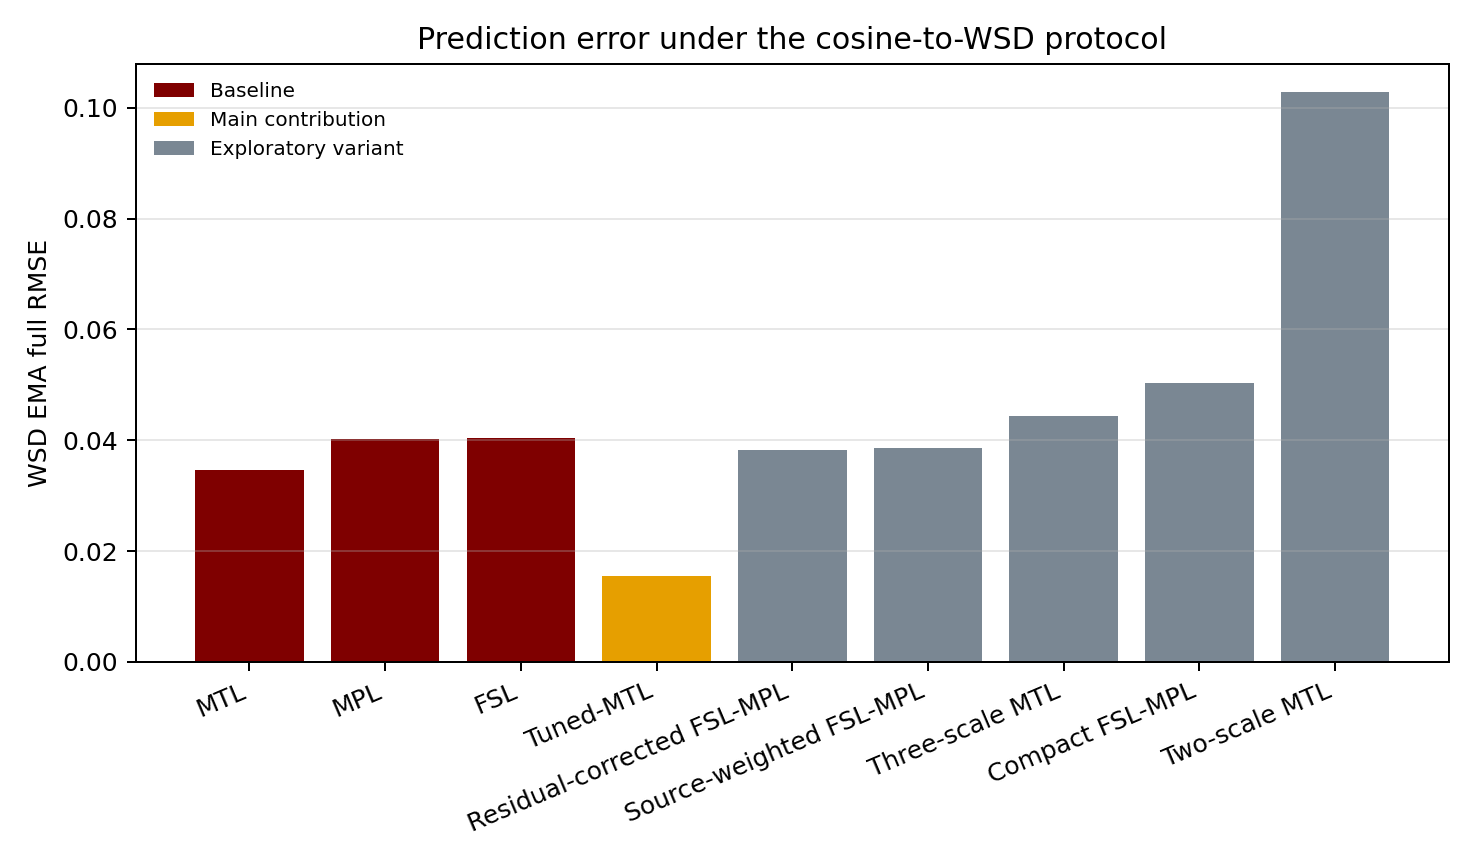
\includegraphics[height=0.62\textheight,keepaspectratio]{all_wsd_rmse_bar.png}
  \end{center}
  \vspace{-0.8em}
  Published baselines appear first, followed by Tuned-MTL and the exploratory variants.
\end{frame}

\begin{frame}{Where Tuned-MTL Gains Accuracy}
  \begin{center}
  \small
  \begin{tabular}{lrr}
    \toprule
    WSD region & Baseline MTL RMSE & Tuned-MTL RMSE \\
    \midrule
    Full evaluation curve & \second{0.034569} & \best{0.015461} \\
    Stable phase & \second{0.037392} & \best{0.007664} \\
    Final 20\% & \best{0.018448} & \second{0.030976} \\
    Final \(1000\) steps & \best{0.004565} & \second{0.020278} \\
    \bottomrule
  \end{tabular}
  \end{center}
  Tuned-MTL's full-curve advantage comes primarily from the long stable phase. Baseline MTL remains more accurate near the endpoint, so the preferred setting depends on the evaluation objective.
\end{frame}

\begin{frame}{Direct Comparison with Baseline MTL}
  \begin{center}
  \small
  \begin{tabular}{lrr}
    \toprule
    Metric & Baseline MTL & Tuned-MTL \\
    \midrule
    WSD RMSE & \second{0.034569} & \best{0.015461} \\
    WSD MAE & \second{0.028816} & \best{0.010069} \\
    WSD MAPE & \second{0.010213} & \best{0.003591} \\
    WSD \(R^2\) & \second{0.963640} & \best{0.992727} \\
    WSD FinalE & \best{0.004317} & \second{0.016741} \\
    WSD WorstE & \best{0.063370} & \second{0.082189} \\
    \bottomrule
  \end{tabular}
  \end{center}
  Tuned-MTL gives the most accurate global trajectory. Baseline MTL provides tighter endpoint and worst-case calibration.
\end{frame}

\begin{frame}{Auxiliary Transfer to the \(8\)-\(1\)-\(1\) Schedule}
  \begin{center}
  \begin{tabular}{lrrr}
    \toprule
    Method & RMSE \(\downarrow\) & MAE \(\downarrow\) & \(R^2\) \(\uparrow\) \\
    \midrule
    MTL & \second{0.030190} & \second{0.024659} & \second{0.973120} \\
    MPL & 0.041732 & 0.030597 & 0.948638 \\
    FSL & 0.041044 & 0.033478 & 0.950317 \\
    \midrule
    Tuned-MTL & \best{0.013594} & \best{0.008491} & \best{0.994550} \\
    \bottomrule
  \end{tabular}
  \end{center}
  \begin{itemize}
    \item Tuned-MTL also attains the lowest error on this second schedule.
    \item Baseline MTL remains the strongest published baseline.
    \item The \(8\)-\(1\)-\(1\) curve is evaluated with the same fitted parameters and metric definitions.
  \end{itemize}
\end{frame}

\begin{frame}{Quantitative Interpretation}
  The results support three conclusions.
  \begin{itemize}
    \item A low-dimensional schedule model is well matched to the one-curve fitting regime.
    \item Memory-scale coverage is decisive: \(\lambda=0.9997\) makes much longer history available to MTL.
    \item Full-curve error and endpoint error reward different calibration choices. Tuned-MTL is strongest for the declared full-region objective, while baseline MTL remains stronger at the final point.
  \end{itemize}
  The auxiliary schedule follows the same overall ranking and strengthens the evidence for the long-memory setting.
\end{frame}

\section{Qualitative Results}

\begin{frame}{Tuned-MTL WSD Prediction}
  \begin{columns}[T,onlytextwidth]
    \begin{column}{0.70\textwidth}
      
\includegraphics[width=\linewidth]{tuned_mtl_wsd_prediction.png}
    \end{column}
    \begin{column}{0.27\textwidth}
      \small
      Tuned-MTL follows the stable WSD phase closely, where its RMSE is \(0.007664\).

      \vspace{0.6em}
      During final decay, the prediction stays above the observed curve. This produces the larger tail and endpoint errors seen in the regional table.
    \end{column}
  \end{columns}
\end{frame}

\begin{frame}{Tuned-MTL Cosine Fit and Transfer}
  \begin{columns}[T,onlytextwidth]
    \begin{column}{0.70\textwidth}
      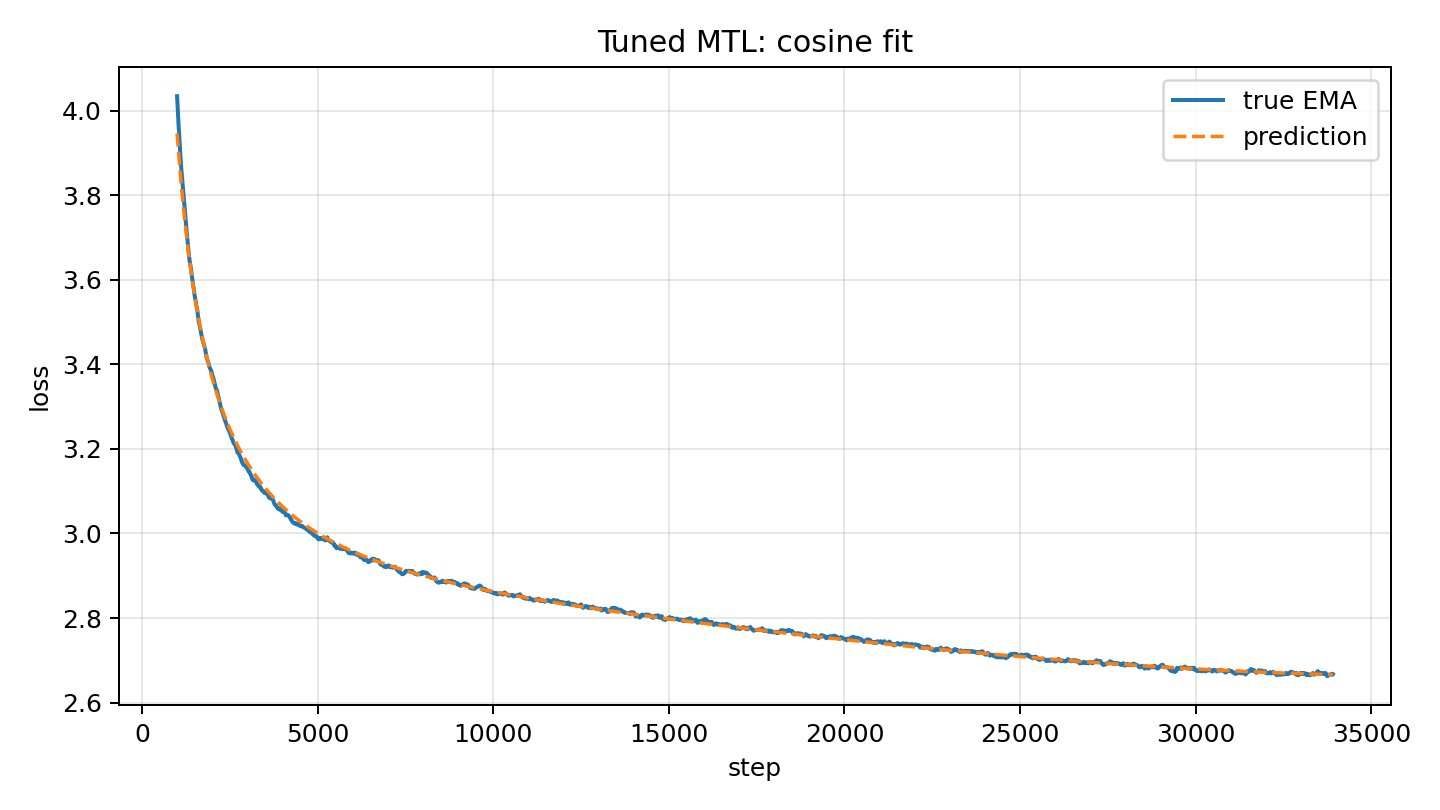
\includegraphics[width=\linewidth]{tuned_mtl_cosine_fit.png}
    \end{column}
    \begin{column}{0.27\textwidth}
      \small
      The fitted cosine curve remains smooth across the full training horizon.

      \vspace{0.6em}
      Tail weighting keeps the fit sensitive to the cosine decay region, while the selected \(\lambda\) supplies the long memory needed for transfer.
    \end{column}
  \end{columns}
\end{frame}

\begin{frame}{Baseline MTL WSD Prediction}
  \begin{columns}[T,onlytextwidth]
    \begin{column}{0.70\textwidth}
      
\includegraphics[width=\linewidth]{mtl_wsd_prediction.png}
    \end{column}
    \begin{column}{0.27\textwidth}
      \small
      Baseline MTL captures the overall WSD shape.

      \vspace{0.6em}
      Its positive bias through much of the stable phase raises full-curve RMSE. Near the endpoint, the prediction converges closely to the observed loss, giving the best FinalE.
    \end{column}
  \end{columns}
\end{frame}

\begin{frame}{Baseline MPL WSD Prediction}
  \begin{columns}[T,onlytextwidth]
    \begin{column}{0.70\textwidth}
      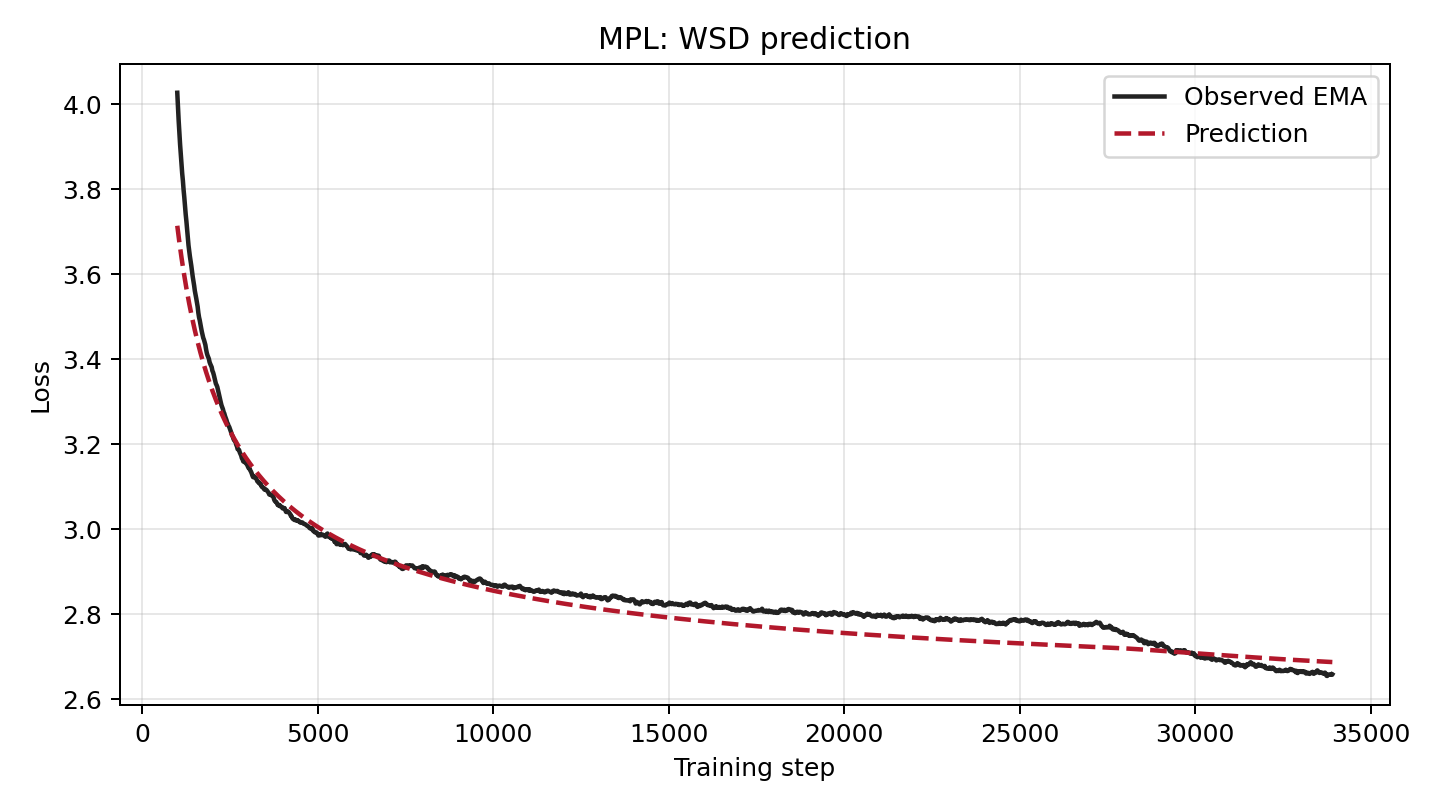
\includegraphics[width=\linewidth]{mpl_wsd_prediction.png}
    \end{column}
    \begin{column}{0.27\textwidth}
      \small
      MPL adapts visibly to the WSD decay transition.

      \vspace{0.6em}
      A large early deviation and a negative bias through the stable phase dominate its full error. The final prediction then moves above the observed curve.
    \end{column}
  \end{columns}
\end{frame}

\begin{frame}{Baseline FSL WSD Prediction}
  \begin{columns}[T,onlytextwidth]
    \begin{column}{0.70\textwidth}
      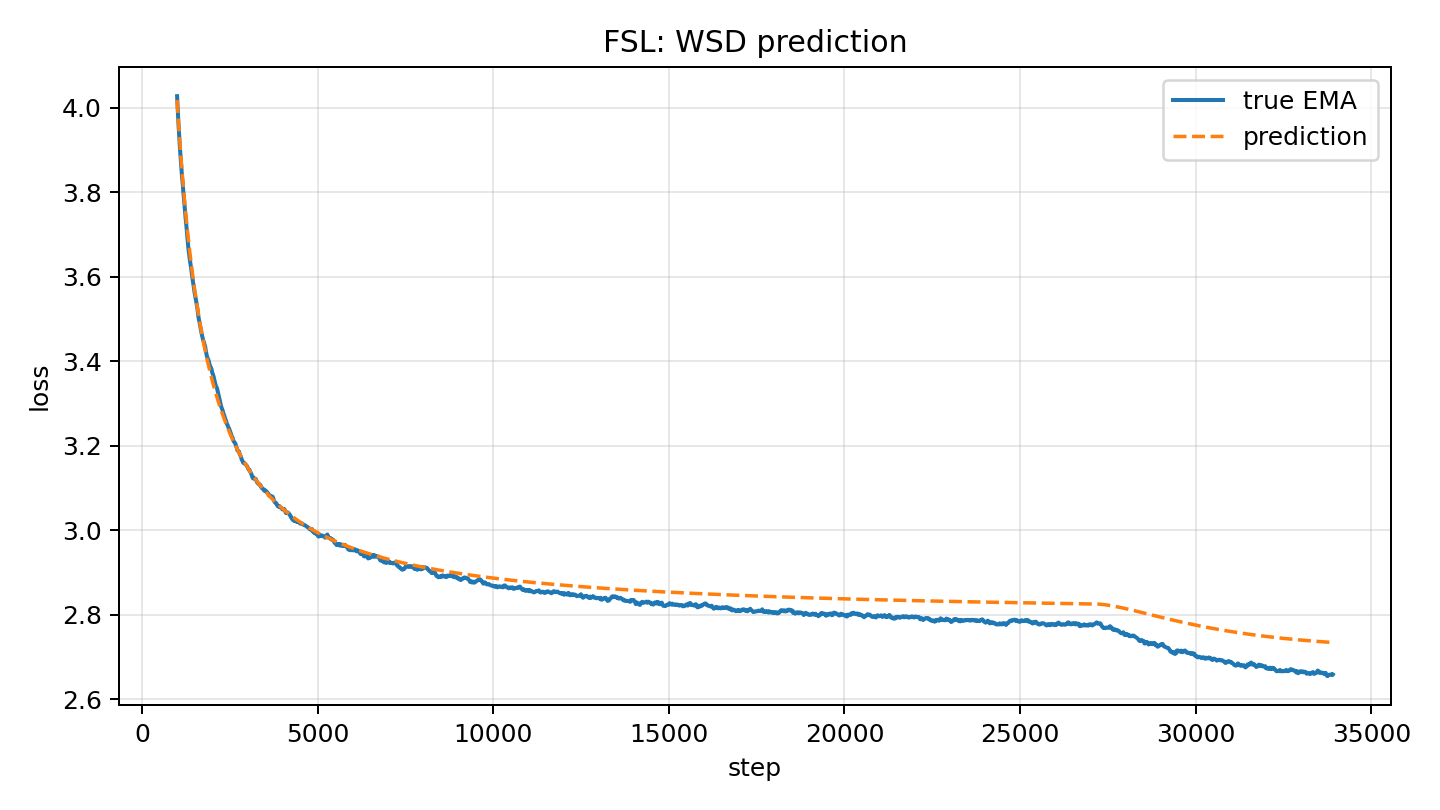
\includegraphics[width=\linewidth]{fsl_wsd_prediction.png}
    \end{column}
    \begin{column}{0.27\textwidth}
      \small
      FSL gives a smooth intrinsic-time prediction.

      \vspace{0.6em}
      It develops a systematic positive bias during WSD decay: the mean decay-region error is \(0.0574\). This bias explains its larger tail and final errors.
    \end{column}
  \end{columns}
\end{frame}

\begin{frame}{Auxiliary Figure: Compact FSL--MPL}
  \begin{columns}[T,onlytextwidth]
    \begin{column}{0.70\textwidth}
      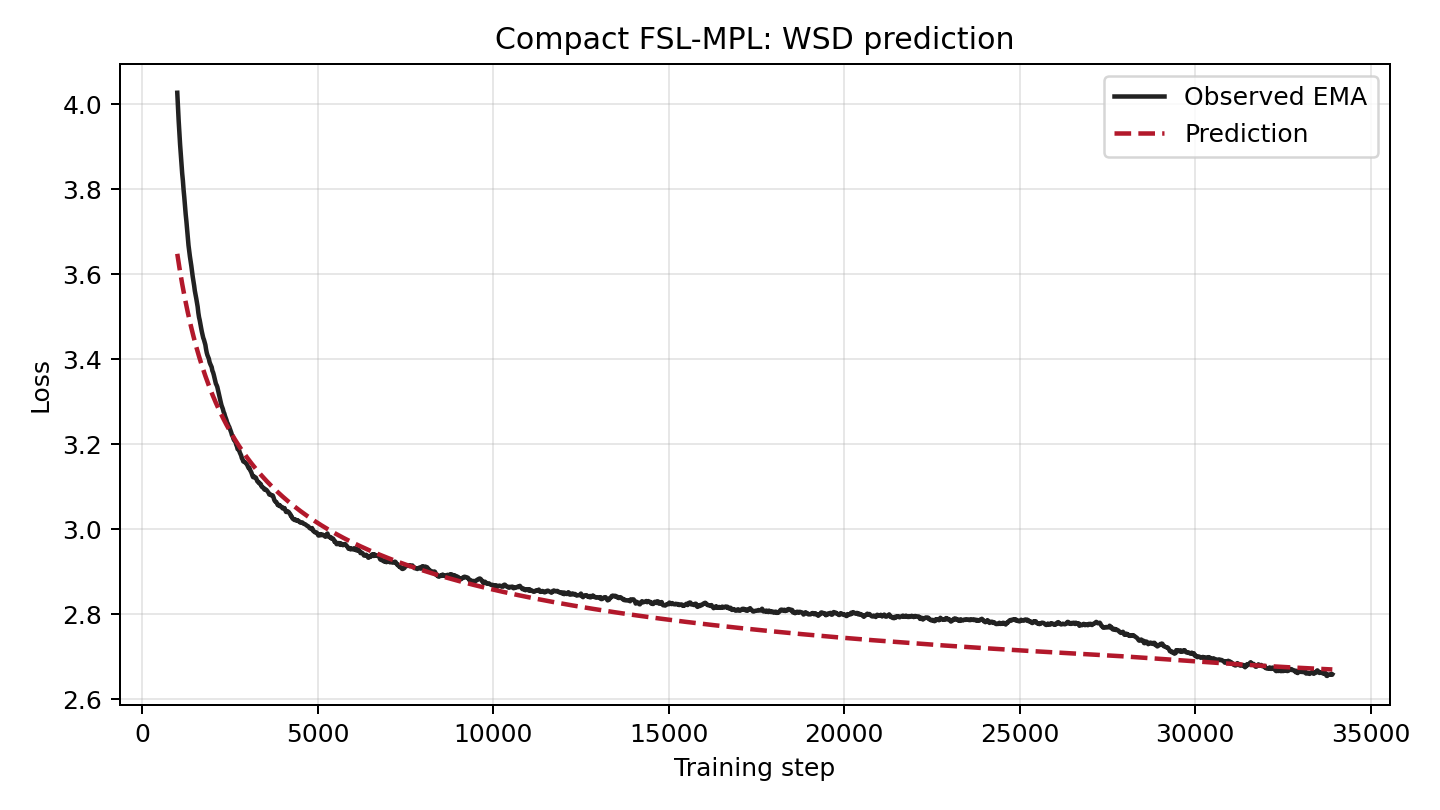
\includegraphics[width=\linewidth]{fslmpl_small_wsd_prediction.png}
    \end{column}
    \begin{column}{0.27\textwidth}
      \small
      This exploratory variant underpredicts much of the stable phase.

      \vspace{0.6em}
      Its endpoint calibration is comparatively strong, although its full-curve RMSE remains above all three published baselines.
    \end{column}
  \end{columns}
\end{frame}

\begin{frame}{Auxiliary Figure: Three-Scale MTL}
  \begin{columns}[T,onlytextwidth]
    \begin{column}{0.70\textwidth}
      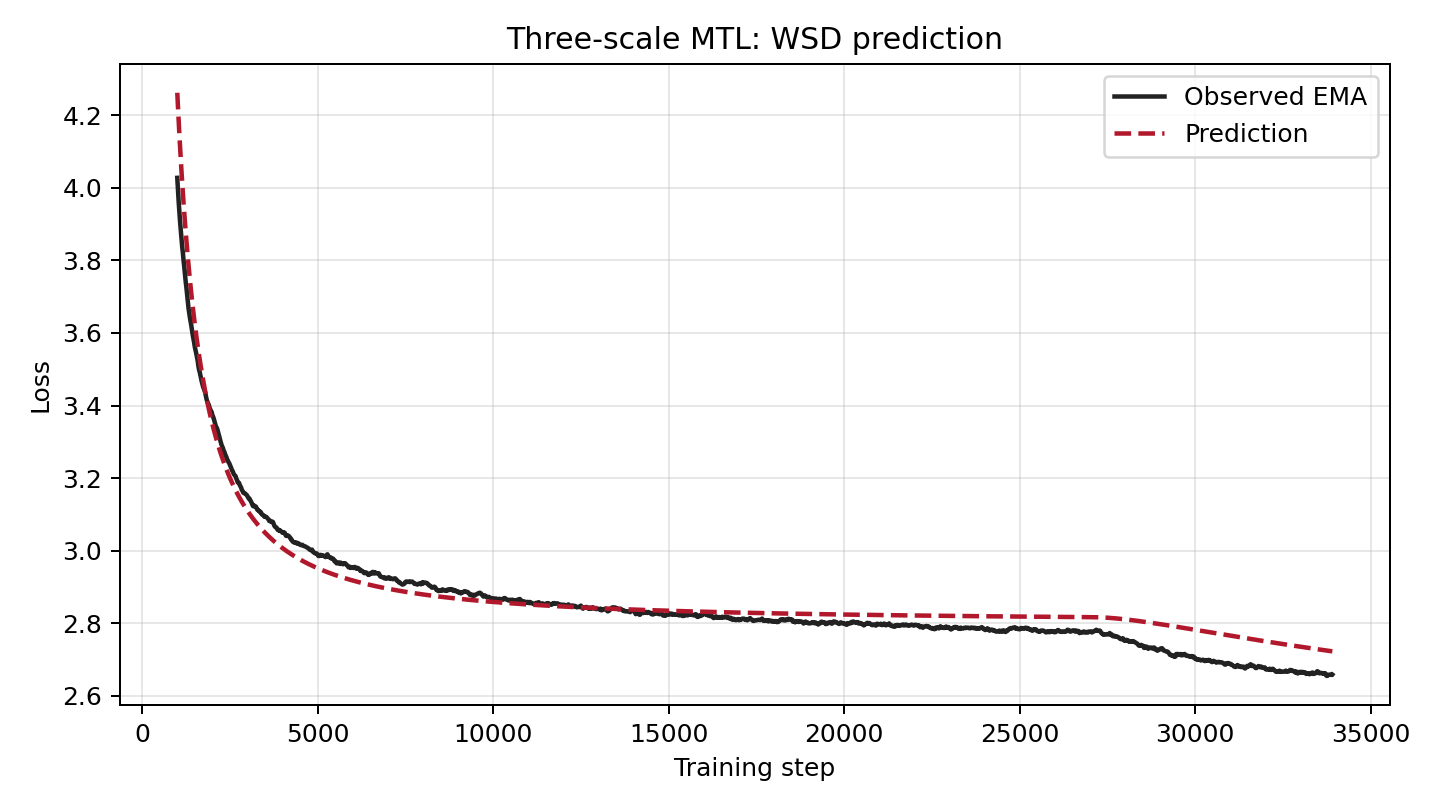
\includegraphics[width=\linewidth]{kmtlm3_wsd_prediction.png}
    \end{column}
    \begin{column}{0.27\textwidth}
      \small
      The three-scale mixture follows the stable region reasonably well.

      \vspace{0.6em}
      It retains too much positive correction through WSD decay, producing a tail RMSE of \(0.0713\). One cosine curve provides limited information for estimating several memory weights.
    \end{column}
  \end{columns}
\end{frame}

\begin{frame}{Qualitative Synthesis}
  The prediction curves clarify the aggregate metrics.
  \begin{itemize}
    \item Tuned-MTL's long memory corrects the broad stable-phase bias that dominates baseline MTL's RMSE.
    \item Baseline MTL forgets schedule changes more quickly and aligns more closely with the final WSD observations.
    \item MPL and FSL respond to decay through richer kernels, yet their fitted responses introduce systematic regional biases.
    \item The auxiliary variants distribute error differently without improving the main full-curve objective.
  \end{itemize}
\end{frame}

\section{Takeaways}

\begin{frame}{Takeaways}
  \begin{itemize}
    \item \textbf{Tuned-MTL is the main contribution.} A broader memory search and stronger late-curve emphasis reduce WSD full-region RMSE by 55.3\% relative to baseline MTL.
    \item The selected \(\lambda=0.9997\) corresponds to a memory half-life of roughly \(2310\) recorded steps, revealing substantial capacity inside the earliest baseline family.
    \item MPL, FSL, and the exploratory variants provide useful alternative inductive biases, while their additional parameters are harder to estimate from one fitting curve.
    \item Metric choice matters: Tuned-MTL leads on the global trajectory, and baseline MTL leads on endpoint calibration.
  \end{itemize}
\end{frame}

\begin{frame}{Scope and Limitations}
  \begin{itemize}
    \item The course dataset contains three curves at one model size and one data budget.
    \item Only the cosine curve is available for continuous parameter fitting, which limits identification of flexible response kernels.
    \item The quantitative conclusions apply to the declared EMA-smoothed, post-warmup, full-region objective.
    \item Broader validation should include additional model sizes, training horizons, and independently generated schedules.
  \end{itemize}
\end{frame}

\begin{frame}{Project Repository}
  We present our project repository at
  \[
    \href{https://github.com/VincentWangzt/TDLT_project}{\textcolor{baselinecolor}{\textbf{https://github.com/VincentWangzt/TDLT\_project}}}.
  \]
  The repository provides:
  \begin{itemize}
    \item the shared data adapter and published baseline implementations;
    \item the Tuned-MTL configuration and the exploratory variants;
    \item fixed-seed experiment entry points and generated prediction tables;
    \item metric definitions, environment specifications, tests, and documentation.
  \end{itemize}
  The README records the complete reproduction procedure and implementation details.
\end{frame}

\begin{frame}{Group Information and Division of Labor}
  \begin{itemize}
    \item Member 1: 黄天域, 学号2300010720, 大三本科生, 实验部分以及前期改进探索
    \item Member 2: 王梓桐, 学号2300010750, 大三本科生, 基线实现以及参数改进探索
    \item Member 3: 柯怿憬, 学号2400013060, 大二本科生, 前期调研, 报告写作, 实验部分
  \end{itemize}
\end{frame}

\appendix
\section{Appendix}

\begin{frame}{Appendix: MTL Memory Grids}
  The baseline search uses
  \[
    \{0.95,\;0.99,\;0.995,\;0.999,\;0.9995\}.
  \]
  Tuned-MTL searches
  \[
  \begin{split}
    \{&0.9,\;0.95,\;0.97,\;0.99,\;0.993,\;0.995,\;0.997,\\
      &0.999,\;0.9993,\;0.9995,\;0.9997,\;0.9999,\;0.99995\}.
  \end{split}
  \]
  The expanded grid resolves long memory scales much more finely near one. The selected value is \(\lambda=0.9997\).
\end{frame}

\begin{frame}{Appendix: Additional Error Definitions}
  For errors \(e_t=\widehat y_t-y_t\):
  \[
    \mathrm{MAPE}
      =\frac{1}{|I|}\sum_{t\in I}\frac{|e_t|}{|y_t|},
    \qquad
    \mathrm{WorstE}
      =\max_{t\in I}|e_t|.
  \]
  Regional RMSE uses the same definition as full RMSE after restricting \(I\):
  \begin{itemize}
    \item \textbf{Stable phase}: observations before the WSD learning rate begins to decay.
    \item \textbf{Final 20\%}: the last fifth of the evaluation interval.
    \item \textbf{Final \(1000\) steps}: observations within \(1000\) steps of the final point.
  \end{itemize}
\end{frame}

\begin{frame}{Appendix: References}
  \footnotesize
  \begin{enumerate}
    \item Howe Tissue, Venus Wang, and Lu Wang. \emph{Scaling Law with Learning Rate Annealing}. 2024. \href{https://arxiv.org/abs/2408.11029}{arXiv:2408.11029}.
    \item Kairong Luo, Haodong Wen, Shengding Hu, Zhenbo Sun, Zhiyuan Liu, Maosong Sun, Kaifeng Lyu, and Wenguang Chen. \emph{A Multi-Power Law for Loss Curve Prediction Across Learning Rate Schedules}. 2025. \href{https://arxiv.org/abs/2503.12811}{arXiv:2503.12811}.
    \item Binghui Li, Fengling Chen, Zixun Huang, Lean Wang, and Lei Wu. \emph{Functional Scaling Laws in Kernel Regression: Loss Dynamics and Learning Rate Schedules}. 2025. \href{https://arxiv.org/abs/2509.19189}{arXiv:2509.19189}.
    \item Huaqing Zhang, Kaiyue Wen, and Tengyu Ma. \emph{Configuration-to-Performance Scaling Law with Neural Ansatz}. 2026. \href{https://arxiv.org/abs/2602.10300}{arXiv:2602.10300}.
  \end{enumerate}
  \vspace{0.35em}
  References 1--3 support the reproduced baseline formulations. Reference 4 motivates the small residual-correction exploration.
\end{frame}

\end{document}
